\subsection{Frequency Branch}

\begin{frame}{Why Add a Frequency Branch?}
  \begin{columns}[T,onlytextwidth]
    \column{.52\textwidth}
      \footnotesize
      \begin{itemize}
        \item Generative models (GANs especially) leave periodic upsampling artifacts, subtle spatially but visible as peaks/asymmetries in the Fourier spectrum.
        \item \textbf{Pipeline:} RGB $\to$ FFT2 $\to$ shift zero-frequency to center $\to$ log-magnitude + phase $\to$ per-channel min-max normalize to $[0,1]$ $\to$ 6-channel input $\to$ small 4-block CNN $\to$ 256-d feature.
        \item Kept lightweight (4 conv blocks, no pretrained backbone): this domain differs too much from ImageNet textures for transfer learning to help.
      \end{itemize}

    \column{.44\textwidth}
      \centering
      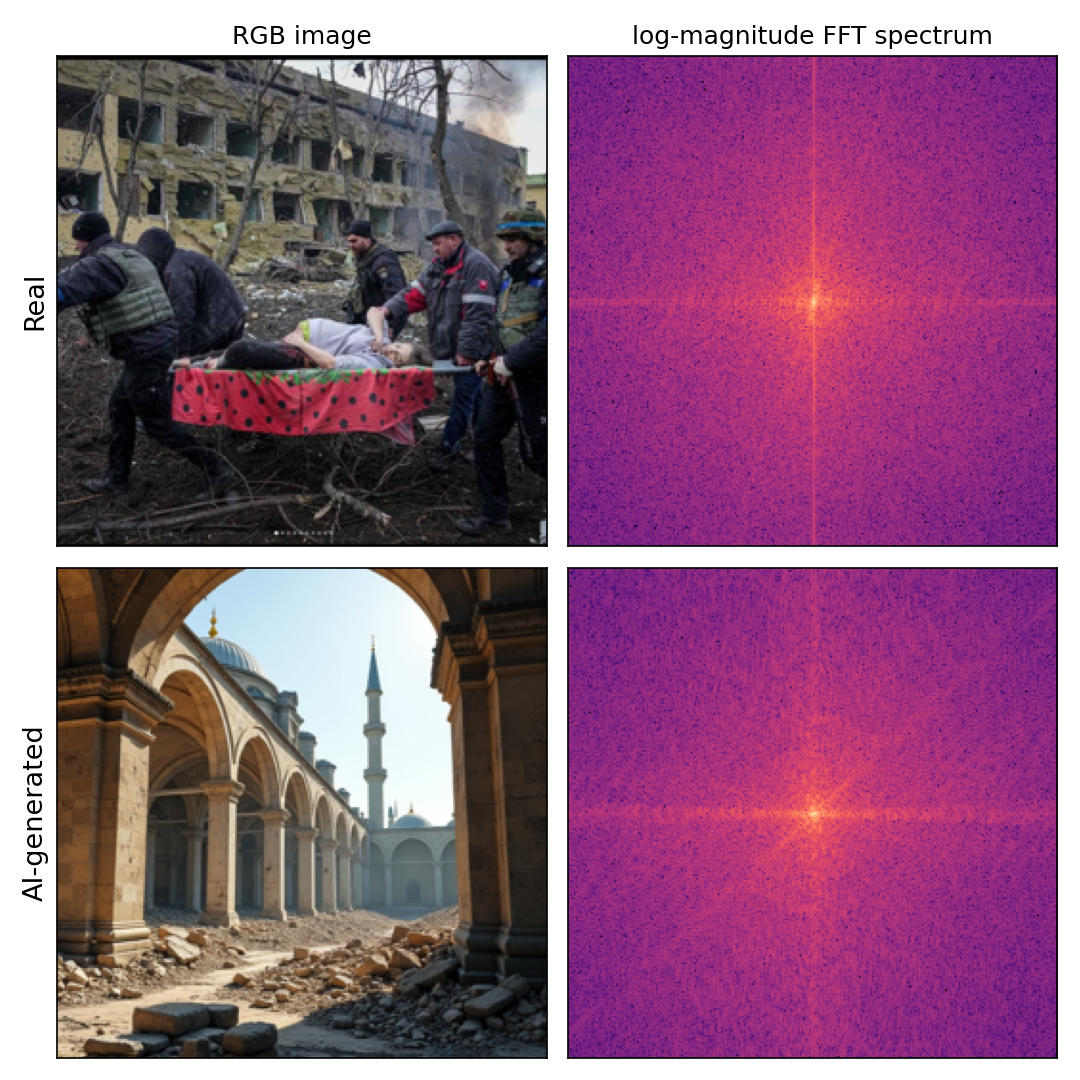
\includegraphics[width=\linewidth]{assets/frequency_spectrum_example.png}\\
      {\scriptsize\color{cookieMuted} RGB vs.\ FFT log-magnitude spectrum}
  \end{columns}
\end{frame}
